\documentclass[a4]{article}

\usepackage[left=3cm,right=3cm,top=2cm,bottom=2cm]{geometry} 

\usepackage[utf8]{inputenc}   % otra alternativa para los caracteres acentuados y la "ñ"
\usepackage[           spanish % para poder usar el español
                      ,es-tabla % para los captions de las tablas
                       ]{babel}   
\decimalpoint %para usar el punto decimal en vez de coma para los números con decimales

\usepackage[T1]{fontenc}
\usepackage{lmodern}

\usepackage{parskip}
\usepackage{xcolor}

\usepackage{caption}

\usepackage{enumerate}% paquete para poder personalizar fácilmente la apariencia de las listas enumerativas

\usepackage{graphicx} % figuras
\usepackage{subfigure} % subfiguras

\definecolor{gris}{RGB}{220,220,220}
	
\usepackage{float} % para controlar la situación de los entornos flotantes

\restylefloat{figure}
\restylefloat{table} 

\newcommand{\HRule}{\rule{\linewidth}{0.5mm}}

\author{David Cabezas Berrido}
\date{\vspace{-5mm}}

\title{\huge Práctica 1: Eficienca \HRule\vspace{-4mm}}

\begin{document}

\maketitle

\tableofcontents

\newpage
\section{Eficiencia Empírica}

\subsection{Algoritmos de ordenación}

\begin{flushleft}
  He medido los tiempos de ejecución de los distintos algoritmos de
  ordenación para varios tamaños de vector, y he obtenido los
  siguientes resultados.
\end{flushleft}

\begin{figure}[!hbp]
  \centering
  \mbox{
    \subfigure[Algoritmos con eficiencia $O(n^2)$]{
      \label{tab:n2}
      \begin{tabular}{| c c c c |}
        \hline
        \multicolumn{1}{|c}{$\textbf{n}$}& \textbf{Burbuja}&
\textbf{Inserción}& \textbf{Selección} \\ \hline
  1000  & 0.004416 & 0.001242 & 0.00132932 \\ 
  2000  & 0.009701 & 0.005147 & 0.00472456 \\ 
  3000  & 0.021534 & 0.012807 & 0.010695   \\ 
  4000  & 0.033732 & 0.020767 & 0.018866   \\ 
  5000  & 0.052993 & 0.024215 & 0.029365   \\ 
  6000  & 0.0785   & 0.034137 & 0.042309   \\ 
  7000  & 0.116606 & 0.046124 & 0.057128   \\ 
  8000  & 0.157316 & 0.059695 & 0.074368   \\ 
  9000  & 0.198552 & 0.074662 & 0.093737   \\ 
  10000 & 0.244325 & 0.092759 & 0.115629   \\ 
  11000 & 0.297715 & 0.11217  & 0.140806   \\ 
  12000 & 0.355768 & 0.13501  & 0.166908   \\ 
  13000 & 0.421353 & 0.157762 & 0.195358   \\
  14000 & 0.490008 & 0.182619 & 0.226432   \\
  15000 & 0.565647 & 0.208906 & 0.260561   \\
  16000 & 0.648838 & 0.239027 & 0.294718   \\
  17000 & 0.734952 & 0.266649 & 0.334074   \\
  18000 & 0.825036 & 0.301845 & 0.373655   \\
  19000 & 0.925171 & 0.334605 & 0.416012   \\
  20000 & 1.02862  & 0.368961 & 0.461119   \\
  21000 & 1.13798  & 0.407094 & 0.508379   \\
  22000 & 1.2548   & 0.448405 & 0.558152   \\
  23000 & 1.37147  & 0.491561 & 0.608983   \\
  24000 & 1.53636  & 0.537183 & 0.662848   \\
  25000 & 1.67428  & 0.586868 & 0.719359   \\ \hline
      \end{tabular}
    }
    
    \qquad

    \subfigure[\vspace{1mm}Algoritmos con eficiencia $O(n\log n)$]{
      \label{tab:nlogn}
      \begin{tabular}{|rlll|} \hline \multicolumn{1}{|c}{$\textbf{n}$}&
\textbf{Mergesort}& \textbf{Quicksort}& \textbf{Heapsort}\\\hline
  1000  & 0.000111503 & 0.000349 & 0.000452 \\ 
  2000  & 0.000235082 & 0.000921 & 0.001106 \\ 
  3000  & 0.000433307 & 0.000349 & 0.001416 \\ 
  4000  & 0.000507335 & 0.000482 & 0.000682 \\ 
  5000  & 0.000711784 & 0.000606 & 0.000806 \\ 
  6000  & 0.000933769 & 0.000764 & 0.000984 \\ 
  7000  & 0.000906519 & 0.00101  & 0.001154 \\ 
  8000  & 0.00109287  & 0.001136 & 0.001349 \\ 
  9000  & 0.0012998   & 0.001303 & 0.001527 \\ 
  10000 & 0.00151355  & 0.001499 & 0.001716 \\ 
  11000 & 0.001805    & 0.001428 & 0.002097 \\ 
  12000 & 0.002079    & 0.001595 & 0.002104 \\ 
  13000 & 0.001935    & 0.001735 & 0.002302 \\
  14000 & 0.001973    & 0.001877 & 0.002499 \\
  15000 & 0.002167    & 0.002125 & 0.002801 \\
  16000 & 0.002389    & 0.002158 & 0.002912 \\
  17000 & 0.002663    & 0.002309 & 0.003118 \\
  18000 & 0.002867    & 0.002161 & 0.003316 \\
  19000 & 0.003284    & 0.002223 & 0.00357  \\
  20000 & 0.003441    & 0.002341 & 0.003735 \\
  21000 & 0.003775    & 0.002306 & 0.003925 \\
  22000 & 0.004023    & 0.002397 & 0.003771 \\
  23000 & 0.004289    & 0.002619 & 0.003569 \\
  24000 & 0.004311    & 0.002889 & 0.003566 \\
  25000 & 0.004956    & 0.002906 & 0.003972 \\ \hline
\end{tabular}
}
}
\end{figure}

\begin{flushleft}
  Puede apreciarse como el tiempo de ejecución de los algoritmos
  $O(n\log n)$ es notablemente menor que el de los algoritmos de orden
  $O(n^2)$. \\
  Dentro de los cuadráticos, el algoritmo de burbuja es notablemente
  peor en todos los casos. Mientras que en los $O(n\log n)$, el
  mergesort es ligeramente peor, y el quicksort es el más eficiente de
  los tres, sobre todo para tamaños grandes.
\end{flushleft}

\newpage
\subsection{Algoritmos de Floyd y Hanoi}

\begin{figure}[!hbp]
  \centering
  \mbox{
    \subfigure[Algoritmos con eficiencia $O(n^3)$]{
      \label{tab:n3}
      \begin{tabular}{| c c |}
        \hline
        \multicolumn{1}{|c}{$\textbf{n}$} & \textbf{Floyd} \\ \hline
        100  & 0.007701 \\ 
        200  & 0.046747 \\ 
        300  & 0.132648 \\ 
        400  & 0.308783 \\ 
        500  & 0.602721 \\ 
        600  & 1.03593  \\ 
        700  & 1.64485  \\ 
        800  & 2.44615  \\ 
        900  & 3.609    \\ 
        1000 & 4.7692   \\ 
        1100 & 6.35587  \\ 
        1200 & 8.29301  \\ 
        1300 & 10.4978  \\
        1400 & 13.1335  \\
        1500 & 16.3889  \\
        1600 & 19.623   \\
        1700 & 23.5916  \\
        1800 & 28.0699  \\
        1900 & 32.8918  \\
        2000 & 38.2142  \\
        2100 & 44.9125  \\
        2200 & 50.9494  \\
        2300 & 58.9452  \\
        2400 & 66.1602  \\
        2500 & 74.5625  \\ \hline
      \end{tabular}
      }

      \qquad

      \subfigure[\vspace{1mm} Algoritmos con eficiencia $O(2^n)$]{
        \label{tab:nlogn}
        \begin{tabular}{| c c |}
          \hline
          \multicolumn{1}{|c}{$\textbf{n}$} & \textbf{Hanoi} \\ \hline
          10 &	2.8e-05  \\
          11 &	5.3e-05  \\
          12 &	0.000101 \\
          13 &	5.4e-05  \\
          14 &	0.000108 \\
          15 &	0.000221 \\
          16 &	0.000457 \\
          17 & 	0.000909 \\
          18 &	0.001828 \\
          19 &	0.003638 \\
          20 &	0.007117 \\
          21 &	0.012896 \\
          22 &	0.025344 \\
          23 &	0.04889  \\
          24 &	0.090453 \\
          25 &	0.181502 \\
          26 &	0.361282 \\
          27 &	0.739665 \\
          28 &	1.43885  \\
          29 &	2.87849  \\
          30 &	5.8083   \\
          31 &	11.5332  \\
          32 &	23.0484  \\
          33 &	46.2319  \\
          34 &	93.0055  \\
          35 &	184.521  \\ \hline
        \end{tabular}
        }
      }
    \end{figure}

    \begin{flushleft}
      Puede apreciarse como los tiempos crecen mucho más rápido que en
      los anteriores algoritmos, sobre todo en el caso de
      Hanoi. Además, he tenido que reducir los rangos de valores para
      que se ejecuten en un tiempo razonable.
    \end{flushleft}

    \section{Gráficos}
    \setcounter{subfigure}{0}

    \begin{flushleft}
      A continuación expongo distintos gráficos donde puede apreciarse
      las comparaciones entre los distintos algoritmos. En cada
      gráfico represento los algoritmos con el mismo orden de
      eficiencia, excepto en el úlimo gráfico, que represento los
      tiempos de todos los algoritmos de ordenación juntos, y puede
      apreciarse cómo los tiempos de los de orden $O(n\log n)$ son
      insignificantes en comparación con los tiempos de los algoritmos
      de orden cuadrático.
    \end{flushleft}

\begin{figure}[H]
  \centering
  \subfigure[Algoritmos con eficiencia
$O(n^2)$]{\label{graf:n2}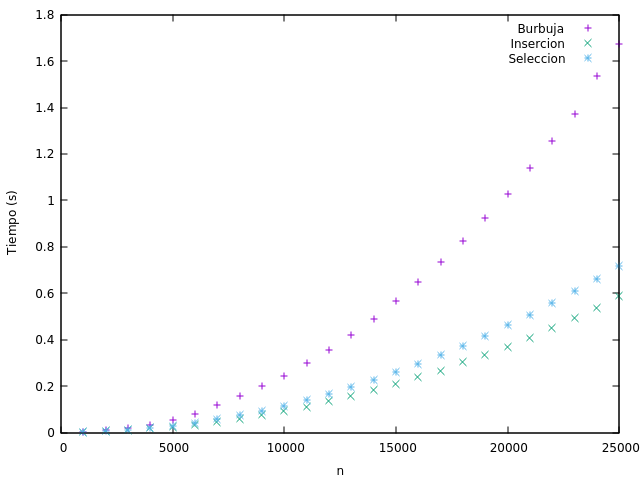
\includegraphics[width=70mm]{graficos/on2}}
\subfigure[Algoritmos con eficiencia $O(n\log
n)$]{\label{graf:nlogn}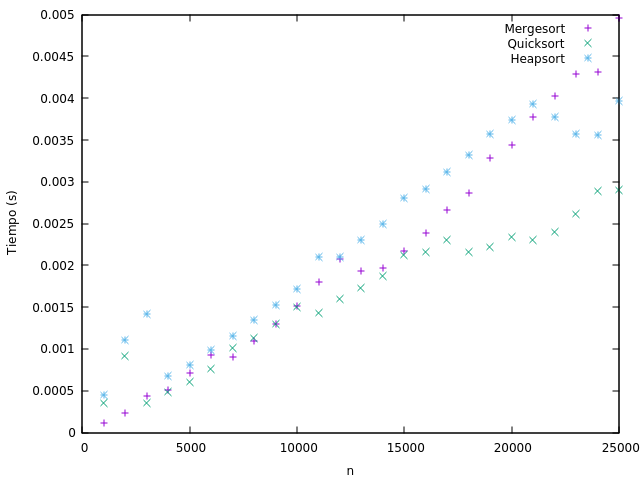
\includegraphics[width=70mm]{graficos/onlogn}}
\subfigure[Algoritmos con eficiencia
$O(n^3)$]{\label{graf:n3}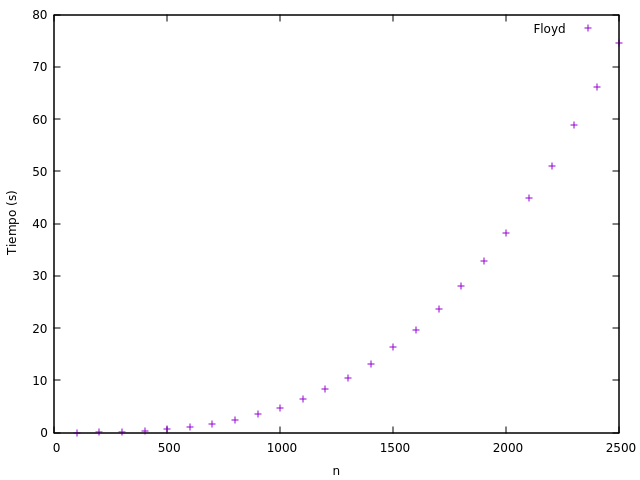
\includegraphics[width=70mm]{graficos/on3}}
\subfigure[Algoritmos con eficiencia
$O(2^n)$]{\label{graf:2n}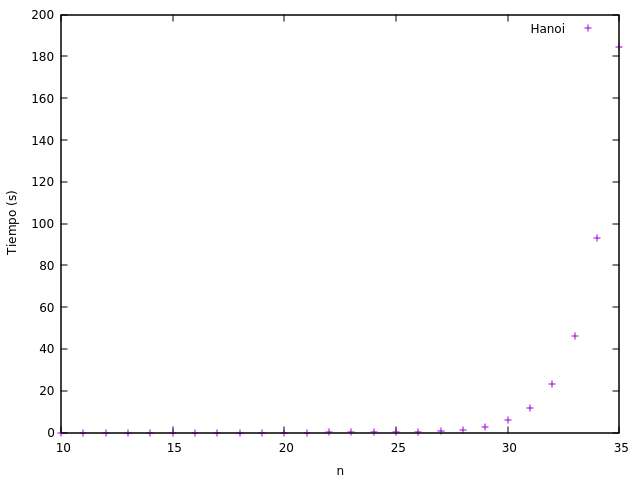
\includegraphics[width=70mm]{graficos/o2n}}
\subfigure[Algoritmos de
ordenación]{\label{graf:sort}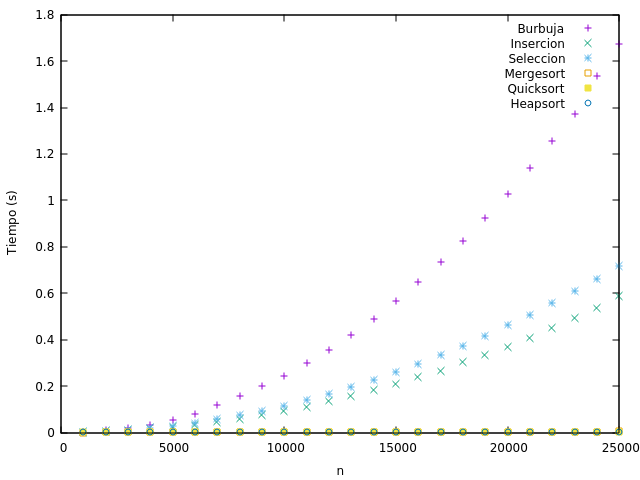
\includegraphics[width=90mm]{graficos/sort}}
\end{figure}

\newpage

\section{Eficiencia Híbrida}
\setcounter{subfigure}{0}

\subsection{Algoritmos con eficiencia $O(n^2)$}

\begin{flushleft}
  Usando la orden \texttt{fit} de \texttt{gnuplot}, he ajustado los
  resultados de estos algoritmos con una función de la
  forma \[\hspace{-30mm}f(x)=a_0x^2+a_1x+a_2\] A continuación expongo
  los distintos coeficientes que he obtenido en el ajuste de los
  tiempos de cada algoritmo, junto con una represención de la función
  y los resultados.
\end{flushleft}

\subsubsection{Burbuja}

\begin{verbatim}
Final set of parameters            Asymptotic Standard Error
=======================            ==========================
a0              = 2.87309e-09      +/- 3.994e-11    (1.39%)
a1              = -6.33841e-06     +/- 1.07e-06     (16.88%)
a2              = 0.014873         +/- 0.006036     (40.59%)
\end{verbatim}

\begin{figure}[H] \centering
\subfigure[\label{graf:ajust-burbuja}Ajuste del algoritmo de
burbuja]{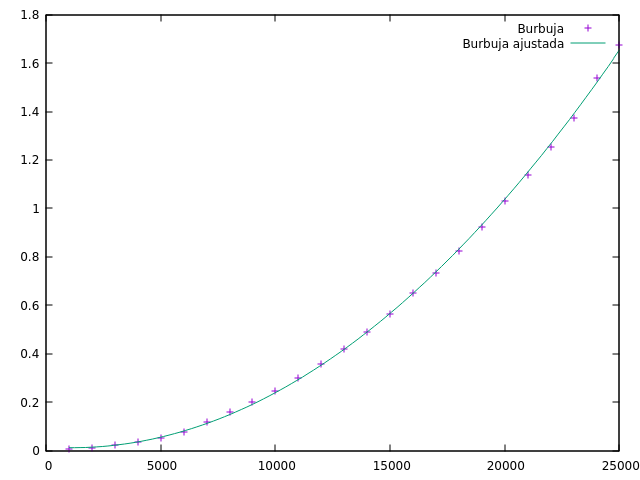
\includegraphics[width=70mm]{graficos/burbuja_ajust}}
\end{figure}

\vspace{-12mm}

\subsubsection{Inserción}

\begin{verbatim}
Final set of parameters            Asymptotic Standard Error
=======================            ==========================
a0              = 9.49226e-10      +/- 8.518e-12    (0.8974%)
a1              = -5.93381e-07     +/- 2.282e-07    (38.45%)
a2              = 0.0039437        +/- 0.001287     (32.64%)
\end{verbatim}

\begin{figure}[H] \centering
\subfigure[\label{graf:ajust-insercion}Ajuste del algoritmo de
inserción]{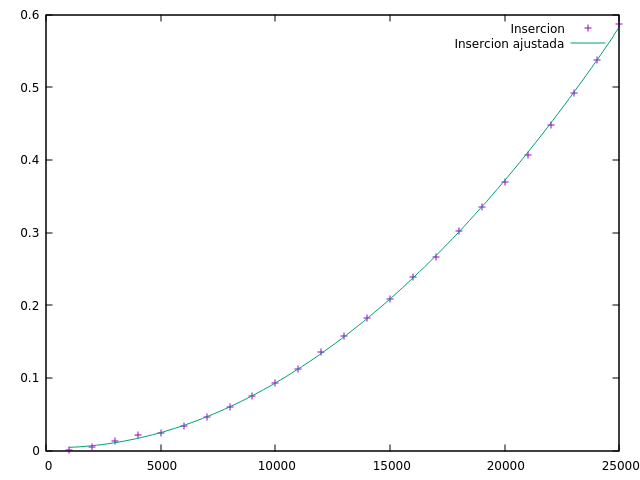
\includegraphics[width=70mm]{graficos/insercion_ajust}}
\end{figure}

\subsubsection{Selección}
\begin{verbatim}
Final set of parameters            Asymptotic Standard Error
=======================            ==========================
a0              = 1.14435e-09      +/- 1.562e-12    (0.1365%)
a1              = 1.72508e-07      +/- 4.185e-08    (24.26%)
a2              = -0.000123672     +/- 0.0002361    (190.9%)
\end{verbatim}

\begin{figure}[H] \centering
\subfigure[\label{graf:ajust-seleccion}Ajuste del algoritmo de
selección]{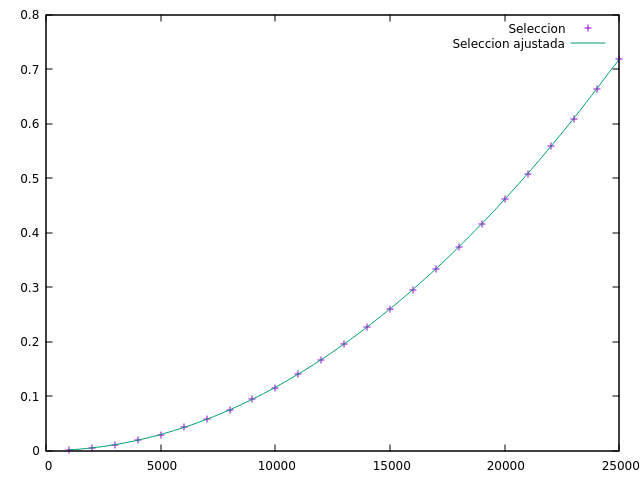
\includegraphics[width=70mm]{graficos/seleccion_ajust}}
\end{figure}

\vspace{-10mm}

\subsection{Algoritmos con eficiencia $O(n\log n)$}

\begin{flushleft}
  Usando la orden \texttt{fit} de \texttt{gnuplot}, he ajustado los
  resultados de estos algoritmos con una función de la
  forma \[\hspace{-30mm}f(x)=ax\log(bx+c)+d\] A continuación expongo
  los distintos coeficientes que he obtenido en el ajuste de los
  tiempos de cada algoritmo, junto con una represención de la función
  y los resultados.
\end{flushleft}

\subsubsection{Mergesort}

\begin{verbatim}
Final set of parameters            Asymptotic Standard Error
=======================            ==========================
a               = 6.95655e-08      +/- 1.431e-08    (20.57%)
b               = 0.000491397      +/- 0.0002775    (56.47%)
c               = 7.18312e-07      +/- 9.373e+04    (1.305e+13%)
d               = 0.000312996      +/- 13.27        (4.239e+06%)
\end{verbatim}

\begin{figure}[H] \centering
\subfigure[\label{graf:ajust-mergesort}Ajuste del algoritmo
mergesort]{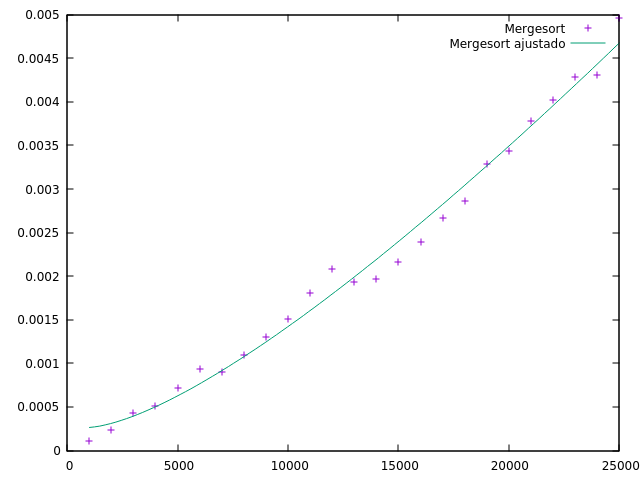
\includegraphics[width=70mm]{graficos/mergesort_ajust}}
\end{figure}

\subsubsection{Quicksort}

\begin{verbatim}
Final set of parameters            Asymptotic Standard Error
=======================            ==========================
a               = 1.07312e-08      +/- 1.716e-08    (159.9%)
b               = 0.542892         +/- 8.438        (1554%)
c               = 7.18316e-07      +/- 2.12e+05     (2.951e+13%)
d               = 0.000390981      +/- 0.004212     (1077%)
\end{verbatim}

\begin{figure}[H]
  \centering
  \subfigure[\label{graf:ajust-quicksort}Ajuste del algoritmo
quicksort]{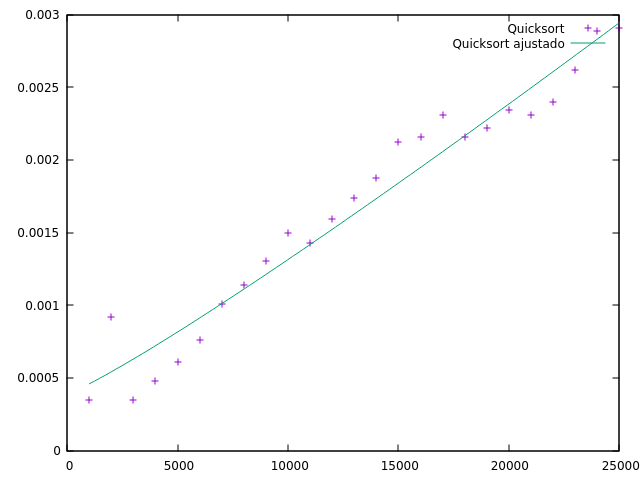
\includegraphics[width=70mm]{graficos/quicksort_ajust}}
\end{figure}

\vspace{-10mm}

\subsubsection{Heapsort}

\begin{verbatim}
Final set of parameters            Asymptotic Standard Error
=======================            ==========================
a               = 2.02343e-08      +/- 2.677e-08    (132.3%)
b               = -0.0611422       +/- 0.6122       (1001%)
c               = 2.74491e-06      +/- 7.44e+05     (2.711e+13%)
d               = 0.000535336      +/- 0.2463       (4.6e+04%)
\end{verbatim}

\begin{figure}[H] \centering
\subfigure[\label{graf:ajust-heapsort}Ajuste del algoritmo
heapsort]{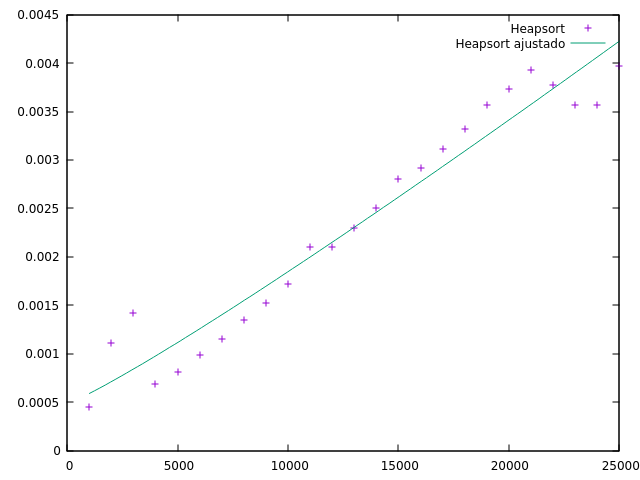
\includegraphics[width=70mm]{graficos/heapsort_ajust}}
\end{figure}

\newpage
\subsection{Algoritmos con eficiencia $O(n^3)$: Floyd}

Usando la orden \texttt{fit} de \texttt{gnuplot}, he ajustado los
resultados de estos algoritmos con una función de la
forma \[\hspace{-30mm}f(x)=a_0x^3+a_1x^2+a_2x+a_3\] A continuación
expongo los distintos coeficientes que he obtenido en el ajuste de los
tiempos de cada algoritmo, junto con una represención de la función y
los resultados.

\begin{verbatim}
Final set of parameters            Asymptotic Standard Error
=======================            ==========================
a0              = 4.6365e-09       +/- 1.322e-10    (2.851%)
a1              = 5.80584e-07      +/- 5.222e-07    (89.94%)
a2              = -0.00053539      +/- 0.0005904    (110.3%)
a3              = 0.111407         +/- 0.1808       (162.3%)
\end{verbatim}

\begin{figure}[H]
  \centering \subfigure[\label{graf:ajust-floyd}Ajuste del algoritmo
  de Floyd]{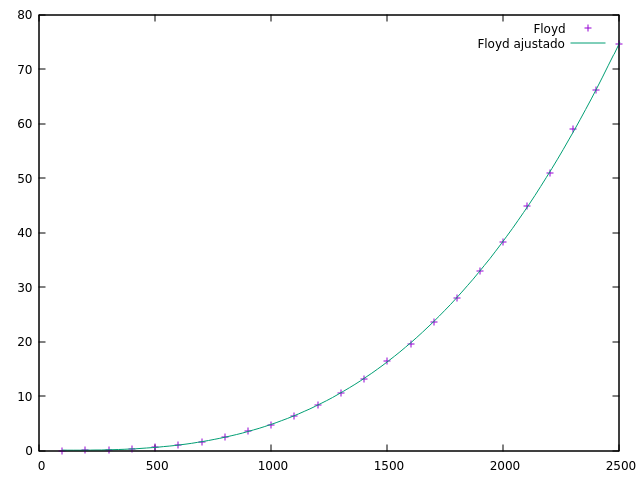
\includegraphics[width=70mm]{graficos/floyd_ajust}}
\end{figure}

\vspace{-12mm}
\subsection{Algoritmos con eficiencia $O(2^n)$: Hanoi}

Usando la orden \texttt{fit} de \texttt{gnuplot}, he ajustado los
resultados de estos algoritmos con una función de la
forma \[\hspace{-30mm}f(x)=a2^x+b\] A continuación expongo los
distintos coeficientes que he obtenido en el ajuste de los tiempos de
cada algoritmo, junto con una represención de la función y los
resultados.

\begin{verbatim}
Final set of parameters            Asymptotic Standard Error
=======================            ==========================
a               = 5.33528e-09      +/- 2.615e-11    (0.49%)
b               = 1                +/- 0.2034       (20.34%)
\end{verbatim}

\vspace{-2mm}

\begin{figure}[H] \centering \subfigure[\label{graf:ajust-hanoi}Ajuste
del algoritmo de
Hanoi]{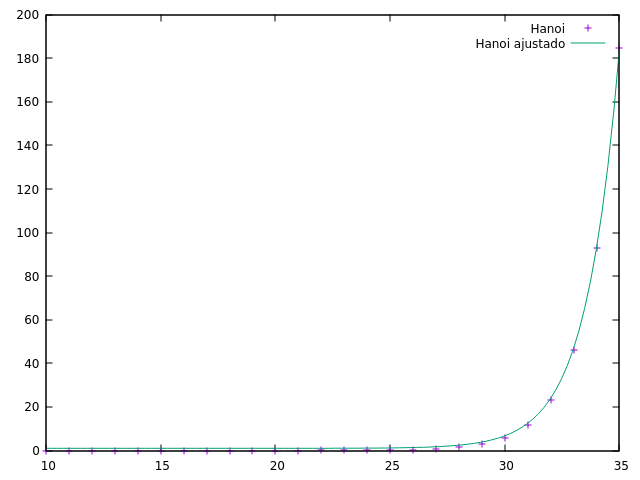
\includegraphics[width=70mm]{graficos/hanoi_ajust}}
\end{figure}

\subsection{Otros ajustes}

\begin{flushleft}
  Tomemos unos ejemplos para ajustar los tiempos de ejecución de un
  algoritmo por una función que no se corresponde con su eficiencia
  teórica.
\end{flushleft}

\subsubsection{Mergesort}

\begin{flushleft} 
  Ajustaremos los tiempos del algoritmo mergesort por tres funciones
  distintas: su eficiencia teórica, un orden inferior y un orden
  superior.
\[f(x)=a_0x\log(a_1x+a_2)+a_3\]
\[g(x)=b_0x+b_1\]
\[h(x)=c_0x^2+c_1x+c_2\]

Según la eficiencia teórica, deberíamos tener un mejor ajuste para $f$
que para $g$ y $h$.
\end{flushleft}

\begin{flushleft}
  Usando \texttt{fit}, he obtenido los siguientes valores para los
  coeficientes de cada función.
\end{flushleft}

\title{Para $f$:}
\begin{verbatim}
final sum of squares of residuals : 3.97491e-07

Final set of parameters            Asymptotic Standard Error
=======================            ==========================
a0              = 6.33118e-06      +/- 0.0005677    (8967%)
a1              = 5.89658e-07      +/- 5.426e-05    (9203%)
a2              = 1.01512          +/- 1.361        (134.1%)
a3              = 0.00010443       +/- 0.0001293    (123.8%)
\end{verbatim}
\title{Para $g$:}
\begin{verbatim}
final sum of squares of residuals : 1.11231e-06

Final set of parameters            Asymptotic Standard Error
=======================            ==========================
b0              = 1.90043e-07      +/- 6.099e-09    (3.209%)
b1              = -0.000322459     +/- 9.067e-05    (28.12%)
\end{verbatim}

\title{Para $h$:}
\begin{verbatim}
final sum of squares of residuals : 3.96375e-07

Final set of parameters            Asymptotic Standard Error
=======================            ==========================
c0              = 3.64724e-12      +/- 5.786e-13    (15.86%)
c1              = 9.52149e-08      +/- 1.55e-08     (16.28%)
c2              = 0.000104267      +/- 8.744e-05    (83.86%)
\end{verbatim}

\newpage

\begin{flushleft}
  En el siguiente gráfico se puede apreciar como $g$ es un mal ajuste
  para los tiempos de este algoritmo, en cambio no se aprecia apenas
diferencia entre $f$ y $h$.
\end{flushleft}

\begin{figure}[H] \centering
\subfigure[\label{graf:otros-mergesort}Diferentes ajustes para el
algoritmo mergesort]{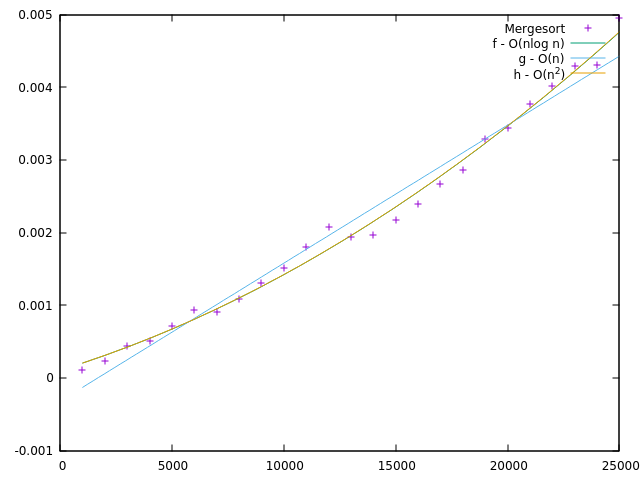
\includegraphics[width=70mm]{graficos/mergesort_otros_ajust}}
\end{figure}

\subsubsection{Hanoi}

\begin{flushleft} 
  Ajustaremos los tiempos del algoritmo de Hanoi por tres funciones
  distintas: su eficiencia teórica, un orden inferior y un orden
  superior.
\[f(x)=a_02^x+a_1\]
\[g(x)=b_0x^{b_1}+b_2\]
\[h(x)=c_03^x+c_1\]

Según la eficiencia teórica, deberíamos tener un mejor ajuste para $f$
que para $g$ y $h$.
\end{flushleft}

\begin{flushleft}
  Usando \texttt{fit}, he obtenido los siguientes valores para los
  coeficientes de cada función.
\end{flushleft}

\title{Para $f$:}
\begin{verbatim}
final sum of squares of residuals : 22.8446

Final set of parameters            Asymptotic Standard Error
=======================            ==========================
a0              = 5.33528e-09      +/- 2.615e-11    (0.49%)
a1              = 1                +/- 0.2034       (20.34%)
\end{verbatim}

\title{Para $g$:}
\begin{verbatim}
final sum of squares of residuals : 154.285

Final set of parameters            Asymptotic Standard Error
=======================            ==========================
b0              = 3.73043e-30      +/- 7.401e-30    (198.4%)
b1              = 20.5177          +/- 0.5393       (2.629%)
b2              = -1.27419         +/- 0.5837       (45.81%)
\end{verbatim}

\title{Para $h$:}
\begin{verbatim}
final sum of squares of residuals : 1736.22

Final set of parameters            Asymptotic Standard Error
=======================            ==========================
c0              = 3.91192e-15      +/- 1.668e-16    (4.264%)
c1              = 1                +/- 1.736        (173.6%)
\end{verbatim}

\begin{flushleft}
  En el siguiente gráfico se puede apreciar como $h$ es un mal ajuste
  para los tiempos de este algoritmo, para ajustar $g$, ha tomado un
  exponente muy alto, aunque aun así tiene un ligero error. En cambio
  $f$ ajusta la gráfica con bastante precisión. Esto se corresponde
  con la suma de los cuadrados de los residuos.
\end{flushleft}

\begin{figure}[H] \centering
  \subfigure[\label{graf:otros-hanoi}Diferentes ajustes para el
  algoritmo de
  Hanoi]{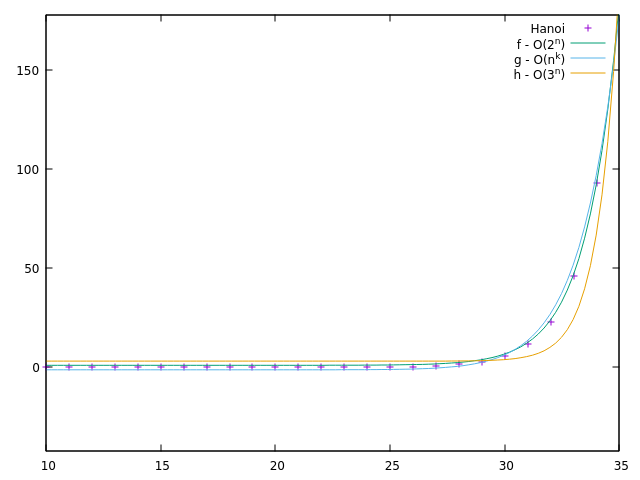
\includegraphics[width=70mm]{graficos/hanoi_otros_ajust}}
\end{figure}

\section{Variación de la eficiencia empírica con parámetros externos}
\setcounter{subfigure}{0}

\begin{flushleft}
  He compilado algunos de los algoritmos con nivel de optimización
  \texttt{O2}, en los siguientes gráficos puede apreciarse como reduce
  el tiempo de ejecución, pero sin afectar al orden de eficiencia.
\end{flushleft}

\begin{figure}[H] \centering
  \subfigure[\label{graf:burbuja-op}Burbuja]{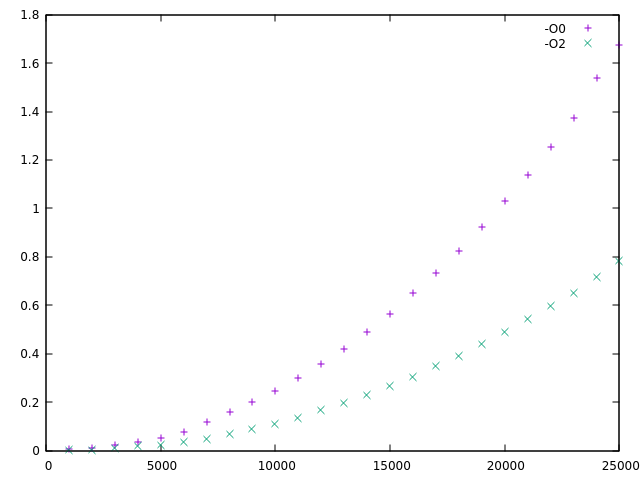
\includegraphics[width=70mm]{graficos/burbuja_op}}
  \subfigure[\label{graf:quicksort-op}Quicksort]{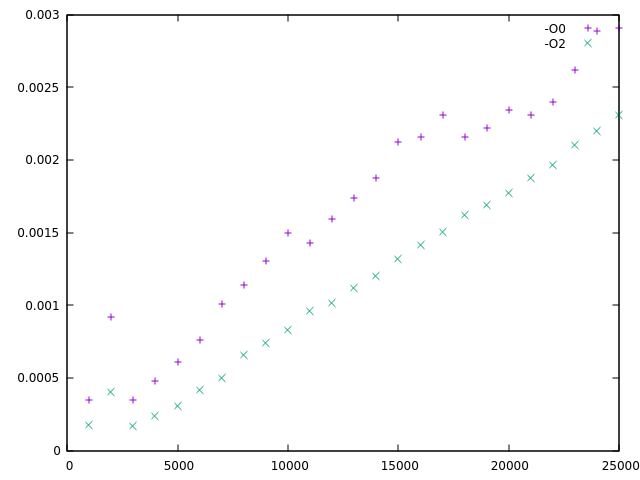
\includegraphics[width=70mm]{graficos/quicksort_op}}
\end{figure}
\vspace{-10mm}
\begin{figure}[H] \centering
  \subfigure[\label{graf:floyd-op}Floyd]{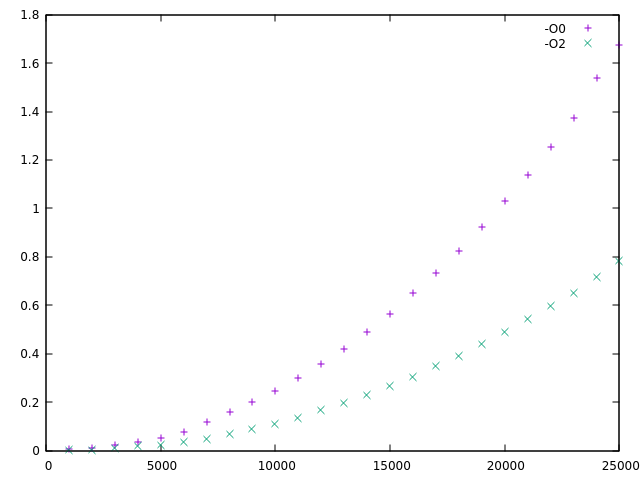
\includegraphics[width=70mm]{graficos/burbuja_op}}
  \subfigure[\label{graf:burbuja-op}Hanoi]{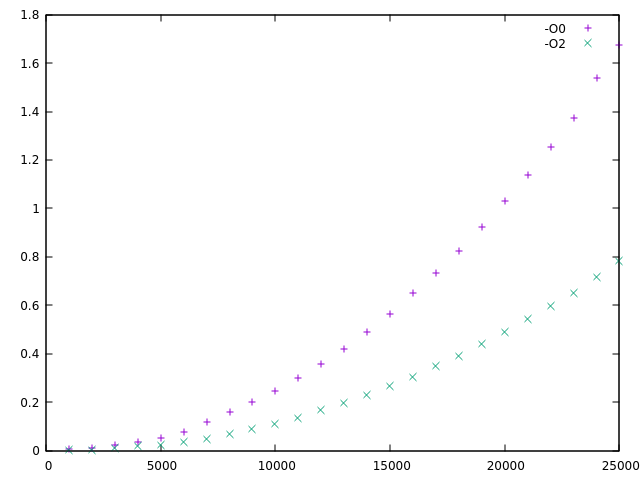
\includegraphics[width=70mm]{graficos/burbuja_op}}
\end{figure}

\end{document}